\documentclass[12pt]{article}

\usepackage{amsmath}
\usepackage{graphicx}
\usepackage{float}

\begin{document}

\title{Exercise: \LaTeX}
\author{Wikipedia \& Asger Gardner}

\maketitle

\section*{i)}

The exponential function is a mathematical function denoted by $f(x)=\text{exp}(x)$ or $e^{x}$ (where the argument x is written as an exponent). It can be defined in several equivalent ways. Its ubiquitous occurrence in pure and applied mathematics led mathematician Walter Rudin to opine that the exponential function is "the most important function in mathematics". 

\section*{ii)}

In this short report, the Taylor-series representation \eqref{eq:taylor_ex} of the exponential function is considered.  

\begin{equation} \label{eq:taylor_ex}
	e^x-1=x+\frac {x^2}2 + \frac{x^3}6+\cdots +\frac{x^n}{n!}+\cdots.	
\end{equation}

Note that in the implementation of this series, only basic arithmetic operations are used when possible in order to circumvent System operations such as Pow(). The Taylor series of any function is an infinite series formulation of the function itself. However, computing an infinite series would require an infinite amount of computations, and would thus run forever on a computer. In order to prevent this unfortunate circumstance, the approximation is only ran until the 10th term in this case. If a negative argument is passed to the function, eg. -x, it is run as $(e^{-x})^{-1}$. If the input argument is of greater precision than 1/8, the function is called recursively as $(e^{\frac{x}{2}})^2$ to maintain the desired precision.

\section*{iii)}

In order to test whether the 10th term Taylor series approximation \eqref{eq:taylor_ex} works, it is compared to the C-sharp system definition, System.Math.Exp. This comparison is shown in figure \ref{fig:ex}. From this figure, it is gathered that \eqref{eq:taylor_ex} is a sufficient approximation. 

\begin{figure}[H] \label{fig:ex}
	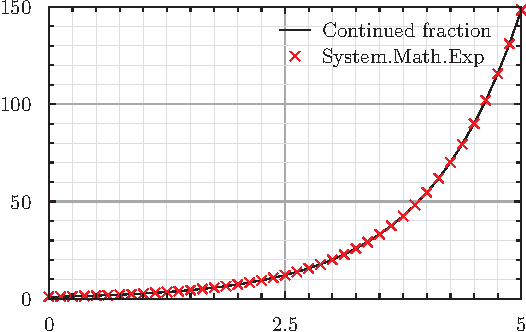
\includegraphics[width=\linewidth]{explot.pdf}
\end{figure}

\end{document}
